\documentclass[11pt,a4paper]{article}

\usepackage[margin=22mm]{geometry}
\usepackage{graphicx}
\usepackage{booktabs}
\usepackage{tabularx}
\usepackage{array}
\usepackage{float}
\usepackage{subcaption}
\usepackage{placeins}
\usepackage{xcolor}
\usepackage{hyperref}
\usepackage{enumitem}

\graphicspath{{fig/}}
\hypersetup{colorlinks=true, linkcolor=blue!55!black, citecolor=blue!55!black, urlcolor=blue!55!black}
\setlist[itemize]{leftmargin=1.4em, itemsep=0.2em}
\setlist[enumerate]{leftmargin=1.5em, itemsep=0.2em}
\newcommand{\mm}{\,\mathrm{mm}}
\newcommand{\m}{\,\mathrm{m}}
\newcommand{\case}[1]{\texttt{\detokenize{#1}}}

\title{\textbf{AutoPos UWB Field Experiment Report}\\
\large OptiTrack-referenced self-localization, static tag localization, and dynamic ROTO validation}
\author{Zekai Xiao}
\date{Erlangen official dataset, 2026-05-28}

\begin{document}
\maketitle

\begin{abstract}
This report summarizes the OptiTrack-referenced UWB results from the Erlangen official dataset collected on 2026-05-28. The main purpose is not to report the smallest number found in the analysis tree, but to identify which result corresponds to the deployable pipeline and which results are ablations, oracle controls, simulations, or future-work evidence. The recommended static deployment headline is the production \case{v4-io/T4} result: $72.7\mm$ median, $171.5\mm$ P95, and $109.8\mm$ RMSE. The dynamic ROTO result for the same original UWB-only configuration is $105.8\mm$ median, $231.8\mm$ P95, and $141.3\mm$ sample RMSE. The most important mechanism result is the delay-layout coupling: OptiTrack anchors without matched delay calibration do not automatically improve localization, while OptiTrack anchors with re-estimated delay reach $77.7\mm$ RMSE. Monte Carlo anchor-dropout tests, wall/NLOS simulations, and preliminary UWB+IMU results are useful for robustness and discussion, but they should not replace the OptiTrack-UWB validation chain as the main experimental claim.
\end{abstract}

\section{Executive Summary}

\begin{table}[H]
\centering
\caption{Recommended headline results. All errors are in mm.}
\begin{tabularx}{\textwidth}{@{}l l r r r X@{}}
\toprule
Block & Configuration & Median & P95 & RMSE & Interpretation \\
\midrule
Static deployed tag localization & \case{v4-io/T4} & 72.7 & 171.5 & 109.8 & Recommended main headline. \\
Static median-estimator ablation & \case{v4-io/T4} & 69.7 & 173.9 & -- & Useful ablation, not the deployed headline. \\
Anchor layout SE(3) rigid alignment & \case{v4-io} vs OptiTrack & -- & -- & 105.4 & Rotation and translation only; this error still includes global scale bias. \\
Anchor layout Sim(3) scale alignment & \case{v4-io} vs OptiTrack & -- & -- & 67.1 & Residual after allowing a global scale factor $s$; estimated scale bias is about $-4.17\%$. \\
Dynamic ROTO original absolute error & \case{v4-io/T4} & 105.8 & 231.8 & 141.3 & Dynamic motion introduces additional error beyond the static case. \\
ROTO post-solve smoothing & F5 & 83.3 & 148.6 & -- & Useful for trajectory presentation, not a calibration result. \\
\bottomrule
\end{tabularx}
\end{table}

The report should make one central claim: \textbf{AutoPos recovers a usable UWB anchor geometry and supports centimeter-to-decimeter tag localization in the measured field setup, but the deployed error is governed jointly by anchor layout, delay calibration, solver choice, dynamic motion, and propagation effects.} This framing avoids overstating ablations or oracle experiments while still showing the strength of the measured system.

\section{Dataset and Evaluation Objects}

The analysis compares three related coordinate or trajectory sources:
\begin{enumerate}
\item \textbf{OptiTrack truth:} reference anchor positions, static tag positions, and dynamic trajectories. It is the evaluation coordinate system, not a deployable input.
\item \textbf{AutoPos UWB self-localized layout:} anchor geometry estimated from UWB measurements. This is the self-deployment capability under test.
\item \textbf{UWB tag localization and ROTO trajectory replay:} tag measurements replayed with different layouts, solvers, delay settings, and filters.
\end{enumerate}

The main deployed configuration in this report is \case{v4-io} for the AutoPos layout and \case{T4} for the production tag solver. Other solvers, filters, Monte Carlo tests, simulated NLOS studies, and Phase 4 UWB+IMU results are treated as controls, robustness evidence, or dynamic-extension material.

\section{Anchor Layout: AutoPos vs OptiTrack}

\begin{figure}[H]
\centering
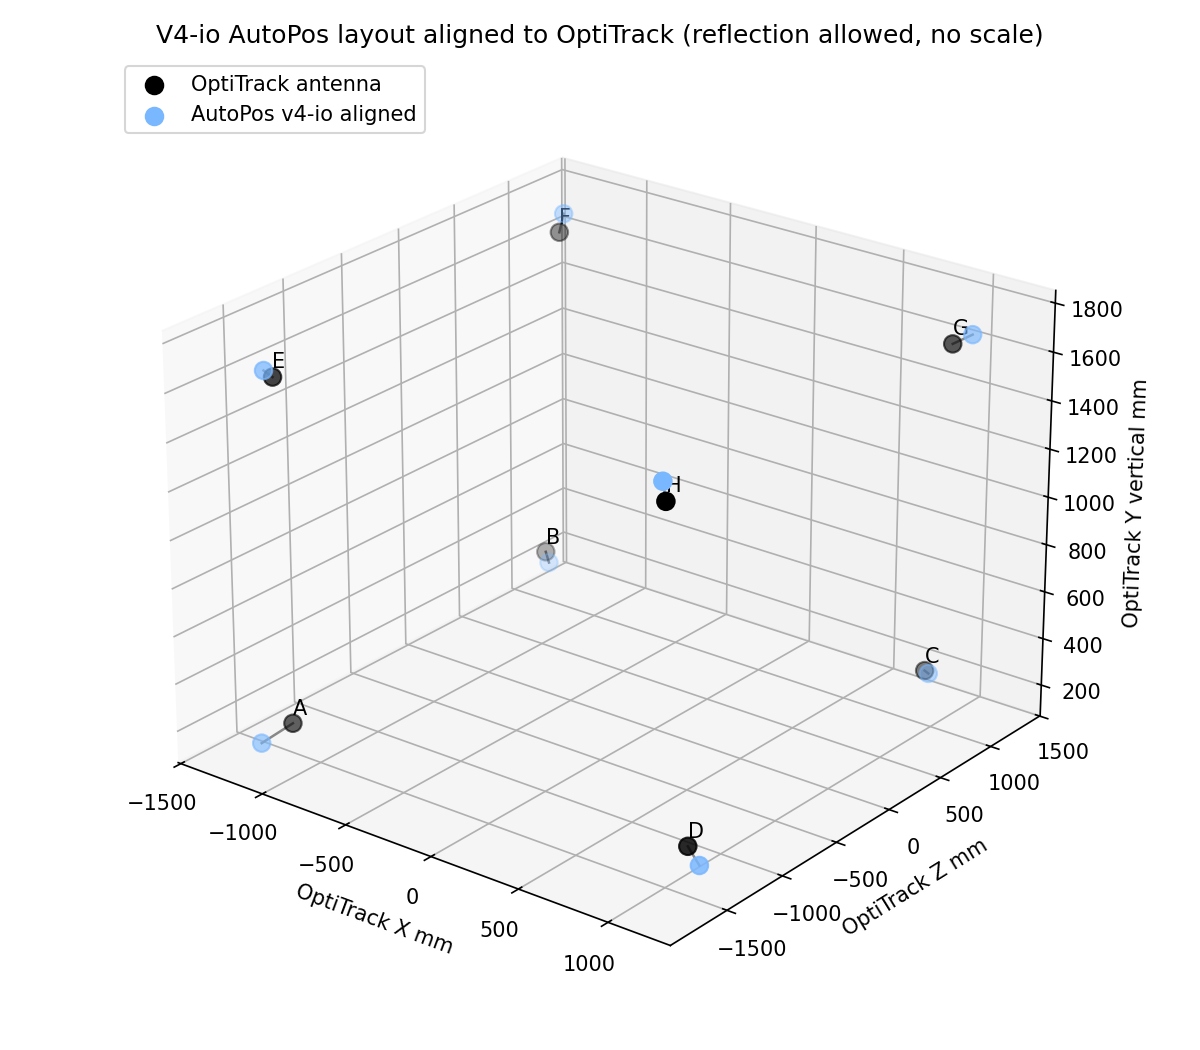
\includegraphics[width=0.78\textwidth]{layout_opti_vs_autopos_3d.png}
\caption{Three-dimensional comparison between the OptiTrack anchor layout and the AutoPos \case{v4-io} layout.}
\end{figure}

The AutoPos \case{v4-io} layout reaches $105.4\mm$ RMSE after rigid SE(3) alignment to the OptiTrack anchor layout. If a Sim(3) scale correction is allowed, the residual drops to $67.1\mm$, with an estimated scale bias of approximately $-4.17\%$. This separation is important: part of the layout discrepancy behaves like global scale or delay-induced bias, while the remaining component is closer to relative anchor-shape error.

The correct interpretation is therefore balanced. AutoPos does not reproduce the OptiTrack layout perfectly, but it does recover a usable spatial structure from real UWB measurements. The absolute scale is coupled to the UWB range-delay model and should be discussed together with delay calibration rather than as a pure geometry error.

\section{Delay-layout Coupling}

\begin{figure}[H]
\centering
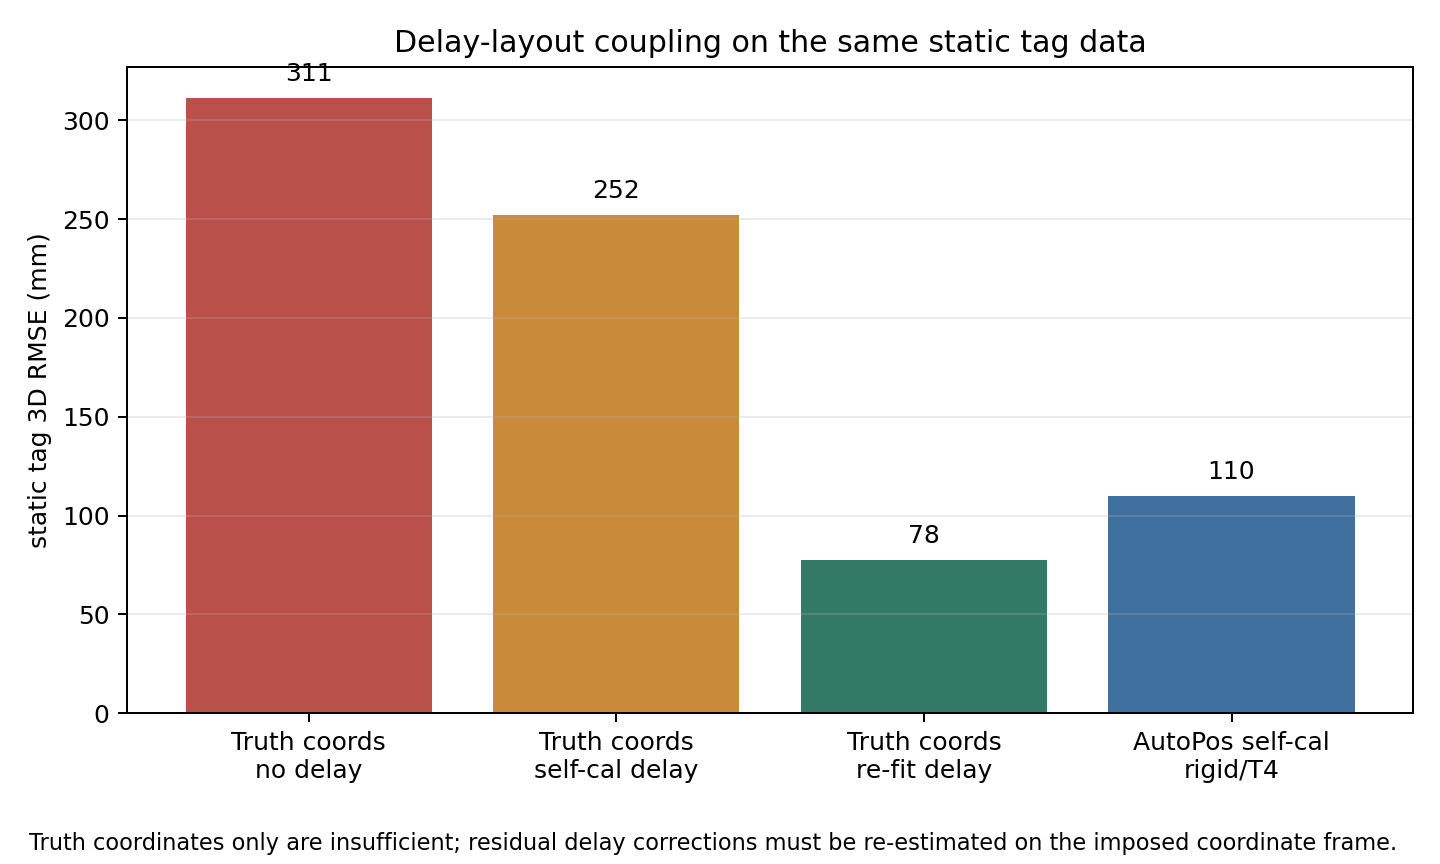
\includegraphics[width=0.78\textwidth]{delay_layout_coupling.png}
\caption{Delay-layout coupling control. Replacing the anchor layout with OptiTrack anchors does not automatically improve localization unless the delay model is also matched to that layout.}
\end{figure}

\begin{table}[H]
\centering
\caption{Delay-layout coupling controls. RMSE values are in mm.}
\begin{tabular}{@{}l r l@{}}
\toprule
Configuration & RMSE & Interpretation \\
\midrule
Vicon anchors, no delay correction & 311.3 & True anchors alone are not enough. Delay dominates. \\
Vicon anchors, transplanted AutoPos delay & 252.2 & Delay parameters are not portable across layouts. \\
Vicon anchors, re-estimated delay & 77.7 & True anchors plus matched delay give strong static performance. \\
AutoPos \case{v4-io}, co-fitted delay & 108.9 & Self-localized layout plus co-fitted delay is deployable. \\
\bottomrule
\end{tabular}
\end{table}

This is the most important mechanism evidence in the report. It shows that anchor layout, UWB delay, and tag solving form a coupled system. The OptiTrack anchor layout is geometrically more accurate, but it can perform poorly if the delay model is not re-estimated for that geometry. Therefore, the main text should not present ``AutoPos versus OptiTrack anchors'' as a one-variable comparison. The proper comparison is layout plus its compatible delay calibration.

\section{Static Tag Localization}

\begin{figure}[H]
\centering
\begin{subfigure}{0.49\textwidth}
\centering
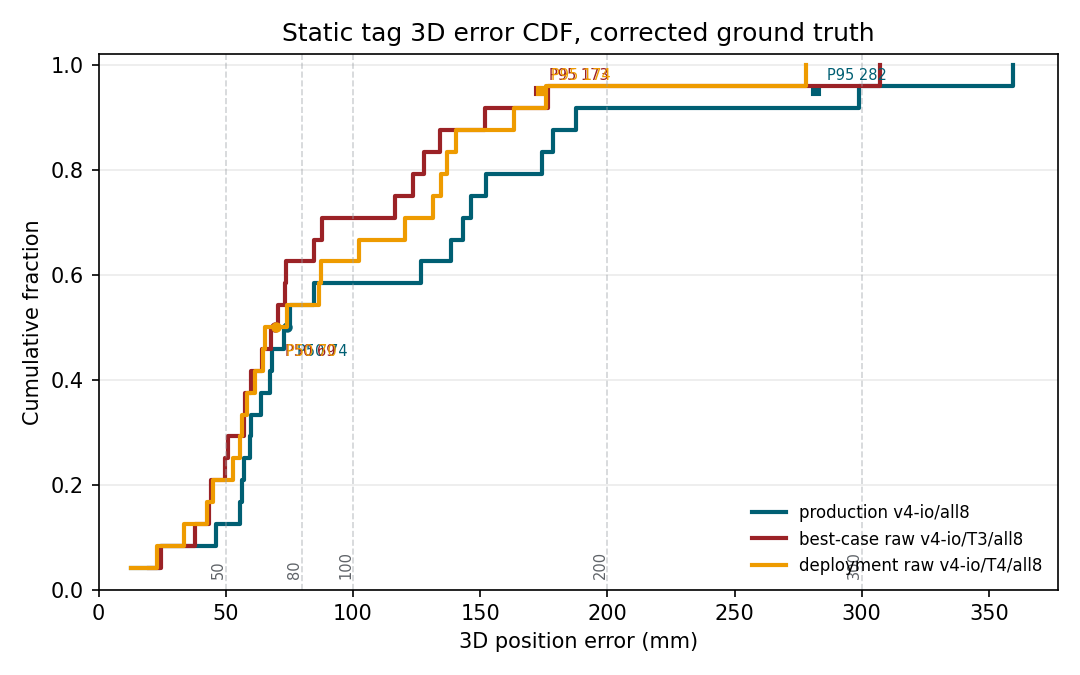
\includegraphics[width=\textwidth]{tag_error_cdf.png}
\caption{Overall error CDF}
\end{subfigure}
\begin{subfigure}{0.49\textwidth}
\centering
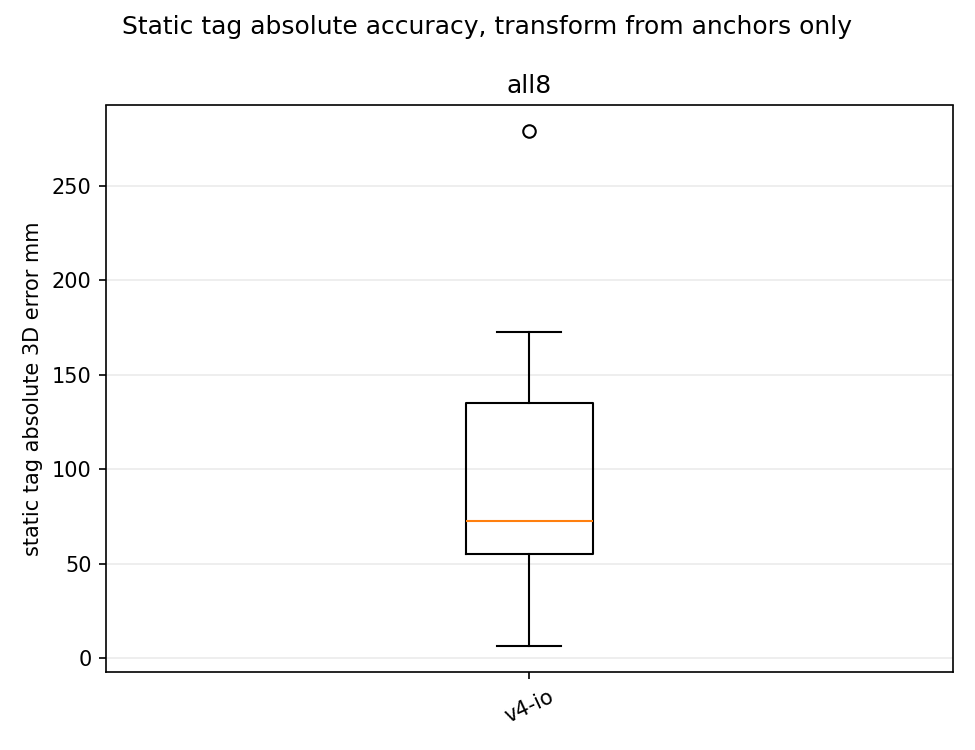
\includegraphics[width=\textwidth]{production_tag_error_by_position.png}
\caption{Production result by position}
\end{subfigure}
\caption{Static tag localization results. The production \case{v4-io/T4} pipeline should be used for the main headline.}
\end{figure}

\begin{figure}[H]
\centering
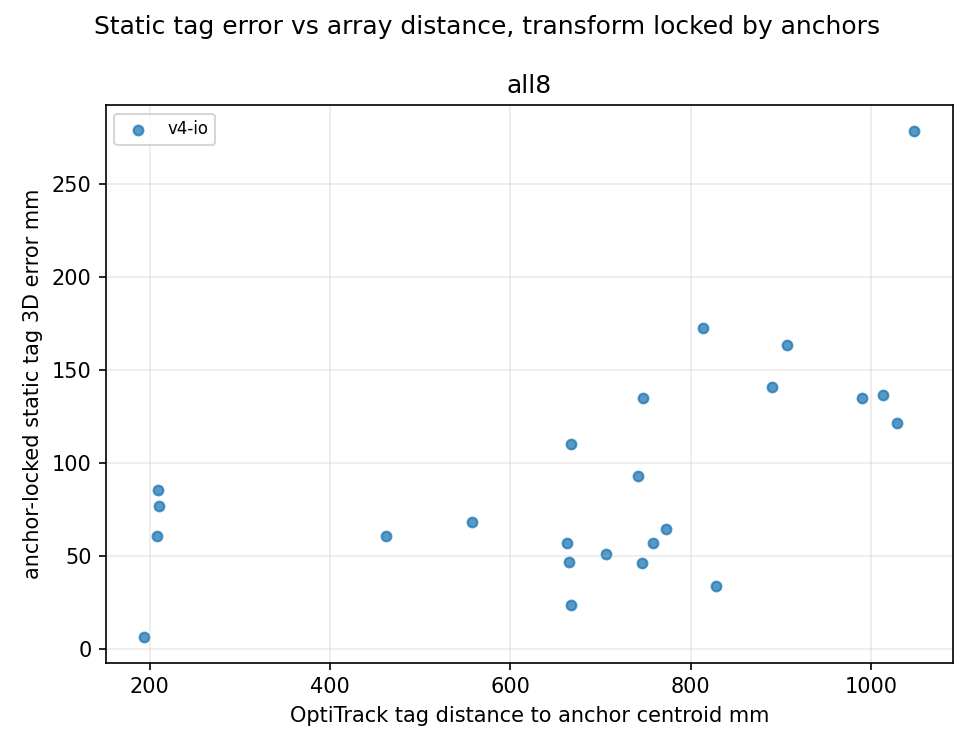
\includegraphics[width=0.72\textwidth]{production_tag_error_vs_distance.png}
\caption{Static production error versus tag-anchor distance. This view is useful for discussing geometry, range-dependent bias, and edge cases.}
\end{figure}

The recommended static localization headline is:
\[
\case{v4-io/T4}: \quad \mathrm{median}=72.7\mm,\quad \mathrm{P95}=171.5\mm,\quad \mathrm{RMSE}=109.8\mm.
\]
This is the deployed production pipeline result and should appear in the abstract, conclusion, and summary table. The smaller $69.7\mm$ median with $173.9\mm$ P95 comes from a median-estimator ablation. It is worth mentioning as an estimator sensitivity result, but it should not be used as the deployed headline.

\subsection{Static Filtering}

\begin{figure}[H]
\centering
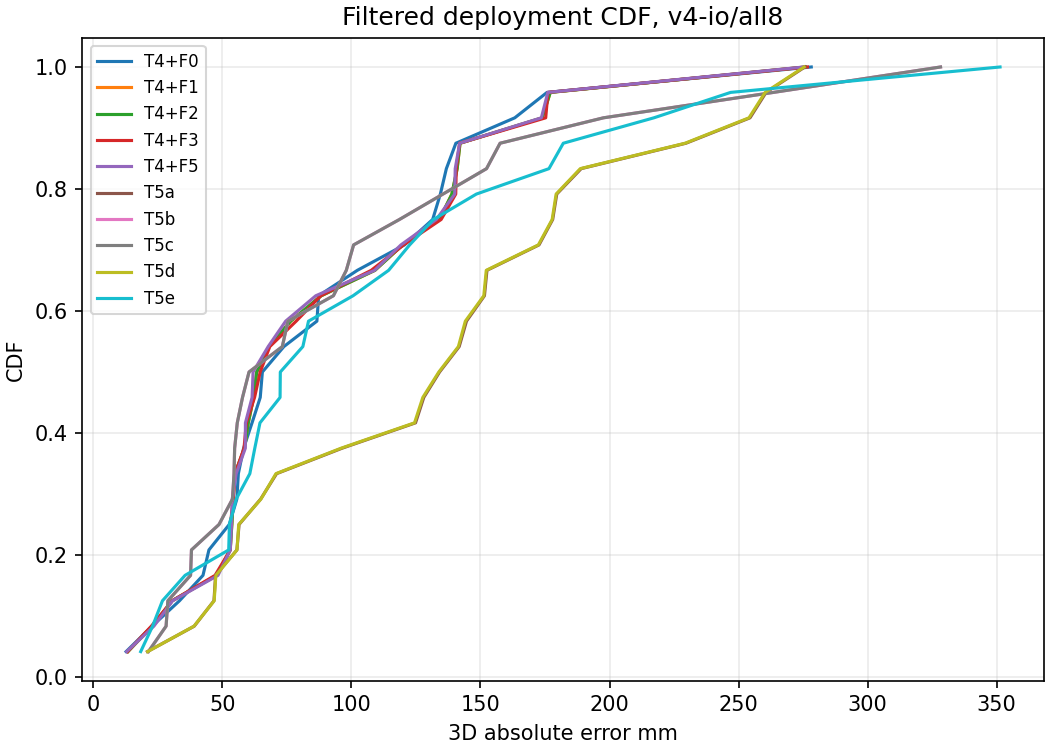
\includegraphics[width=0.75\textwidth]{filtered_static_cdf_v4io_all8.png}
\caption{Static filtered deployment CDF for \case{v4-io}. F5 improves repeatability but does not remove systematic bias.}
\end{figure}

Static lock/filter F5 reduces repeatability spread from $67.4\mm$ to $18.7\mm$. This is useful for steady displays or slow-updating static use cases, but it should not be presented as a correction of anchor layout or delay calibration. Filtering mainly suppresses random variation; fixed bias remains a separate issue.

\section{Dynamic ROTO Evaluation}

\begin{figure}[H]
\centering
\begin{subfigure}{0.49\textwidth}
\centering
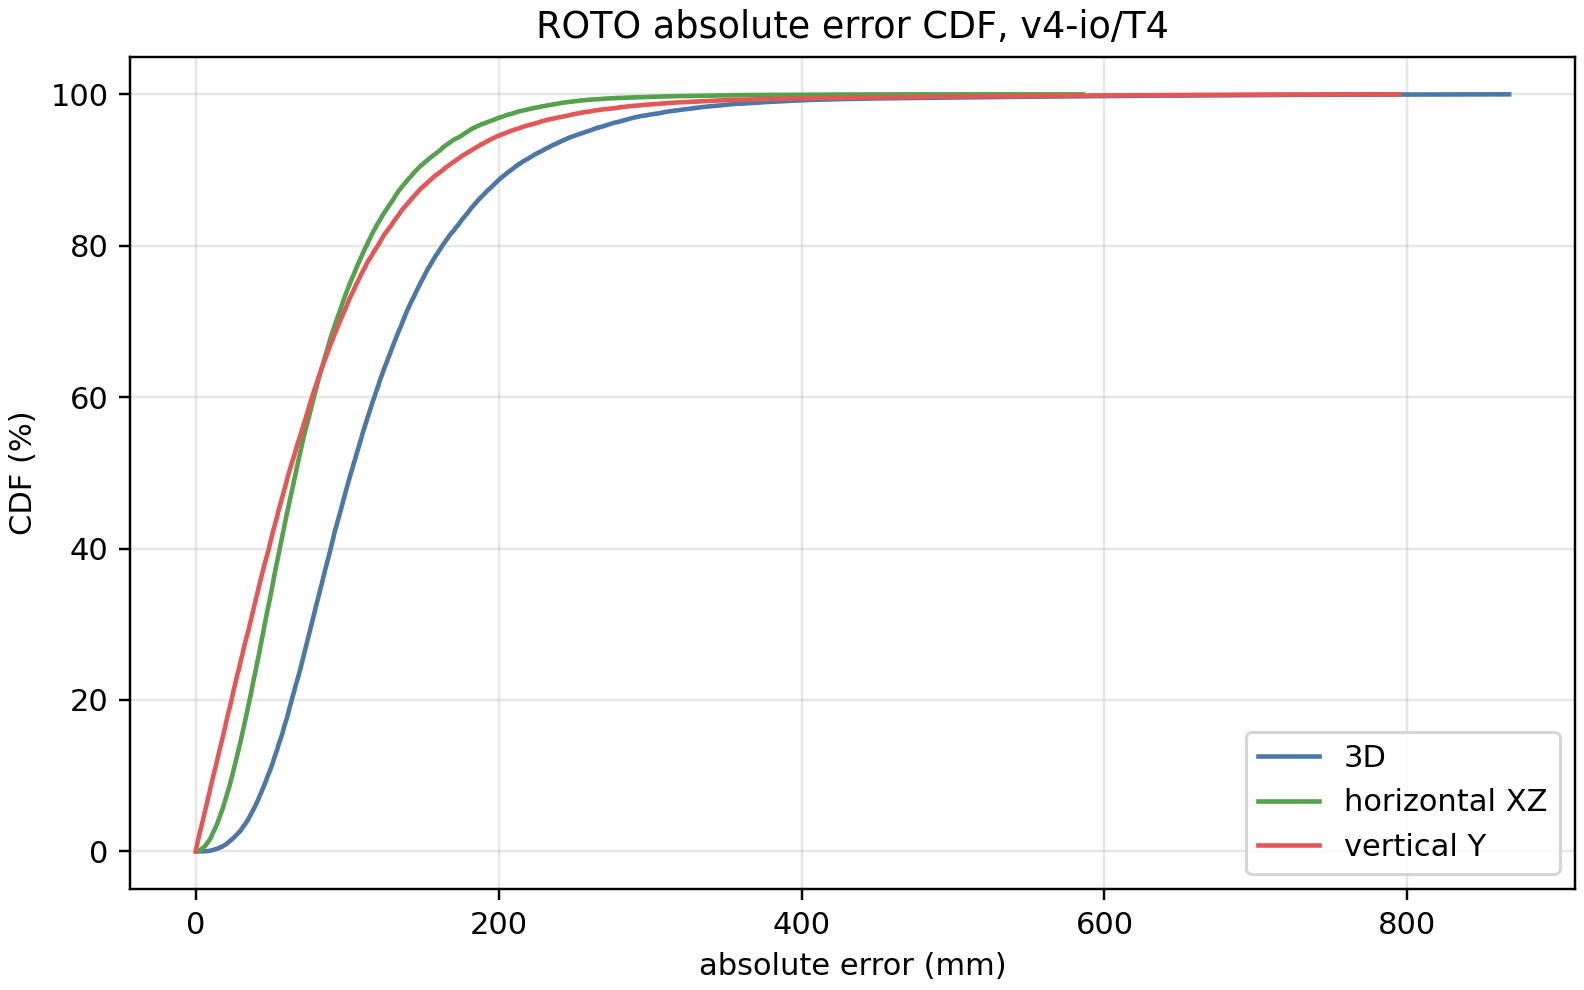
\includegraphics[width=\textwidth]{roto_abs_cdf_v4io_T4.png}
\caption{ROTO absolute error CDF}
\end{subfigure}
\begin{subfigure}{0.49\textwidth}
\centering

\includegraphics[width=\textwidth]{roto_solver_matrix_median3d.png}
\caption{ROTO solver matrix}
\end{subfigure}
\caption{Dynamic ROTO results. The dynamic error is higher than the static deployed result, indicating additional motion-dependent error sources.}
\end{figure}

\begin{figure}[H]
\centering
\begin{subfigure}{0.49\textwidth}
\centering
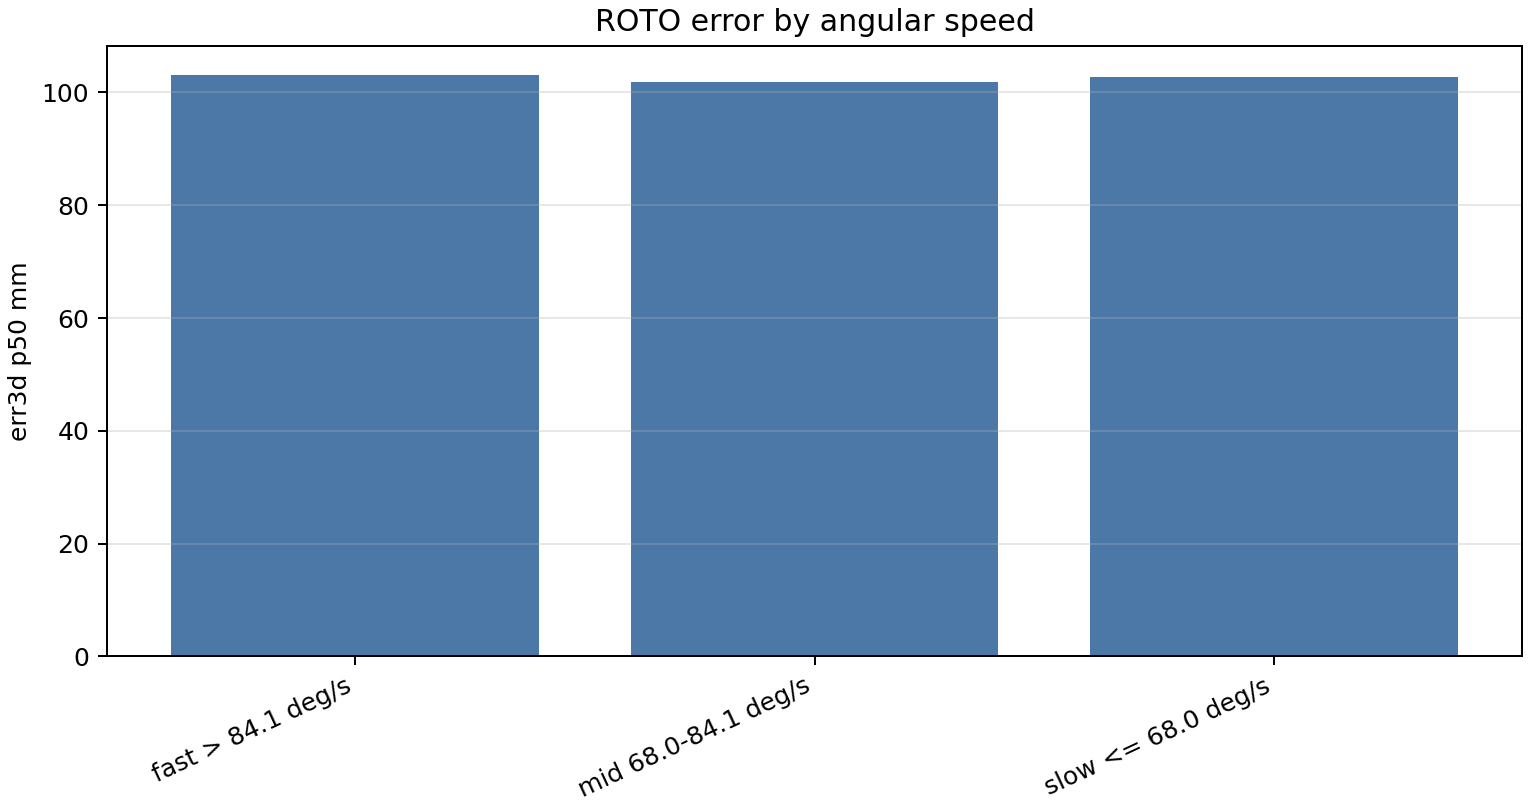
\includegraphics[width=\textwidth]{roto_error_by_angular_speed.png}
\caption{Error by angular speed}
\end{subfigure}
\begin{subfigure}{0.49\textwidth}
\centering
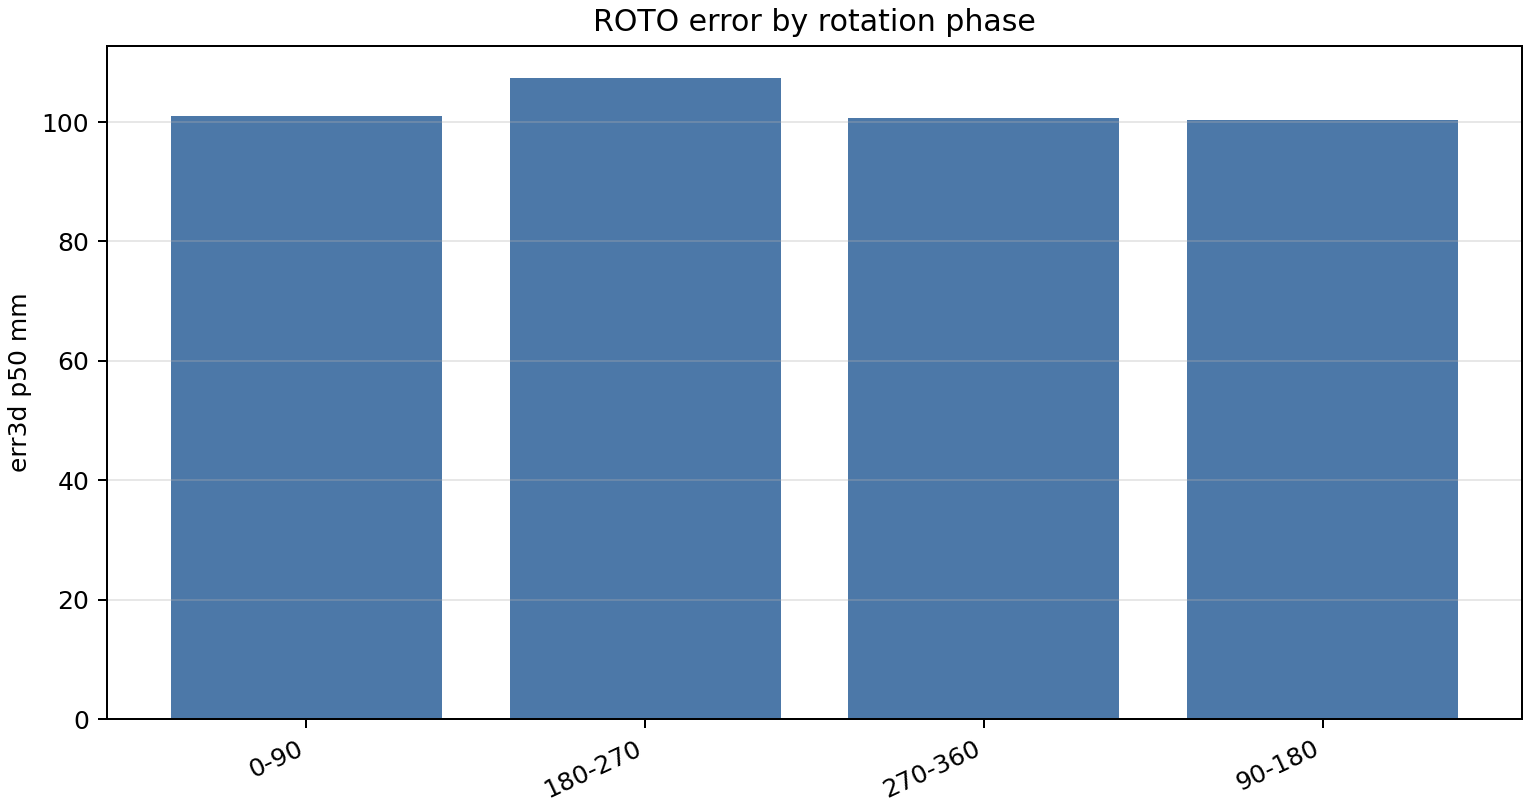
\includegraphics[width=\textwidth]{roto_error_by_phase.png}
\caption{Error by motion phase}
\end{subfigure}
\caption{ROTO diagnostics. These figures support the interpretation that dynamic ROTO error is not just a static layout bias.}
\end{figure}

For the original UWB-only \case{v4-io/T4} configuration, ROTO reaches $105.8\mm$ median, $231.8\mm$ P95, and $141.3\mm$ sample RMSE. Even after replacing the layout with Vicon anchors and re-estimating delay, the ROTO result remains about $105.6\mm$ median and $200.4\mm$ P95. This negative result is scientifically useful: the dynamic error is not solved by anchor-layout replacement alone.

Timing checks point in the same direction. Clock skew changes pooled P50 by only about $0.11\mm$, and a $0.8\mathrm{ms}$ protocol window corresponds to only about $0.5$--$0.7\mm$ of motion in the measured setup. The hundred-millimeter ROTO tail is therefore more plausibly caused by dynamic range bias, body shadowing, antenna orientation, multipath/NLOS, and solver motion assumptions.

Post-solve ROTO filters can improve visual smoothness and final trajectory metrics: F4 reaches about $86.3\mm$ median and $158.2\mm$ P95, while F5 reaches about $83.3\mm$ median and $148.6\mm$ P95. These should be described as smoothers, not as calibration results.

\section{Monte Carlo Keep-k Robustness}

\begin{figure}[H]
\centering
\begin{subfigure}{0.49\textwidth}
\centering
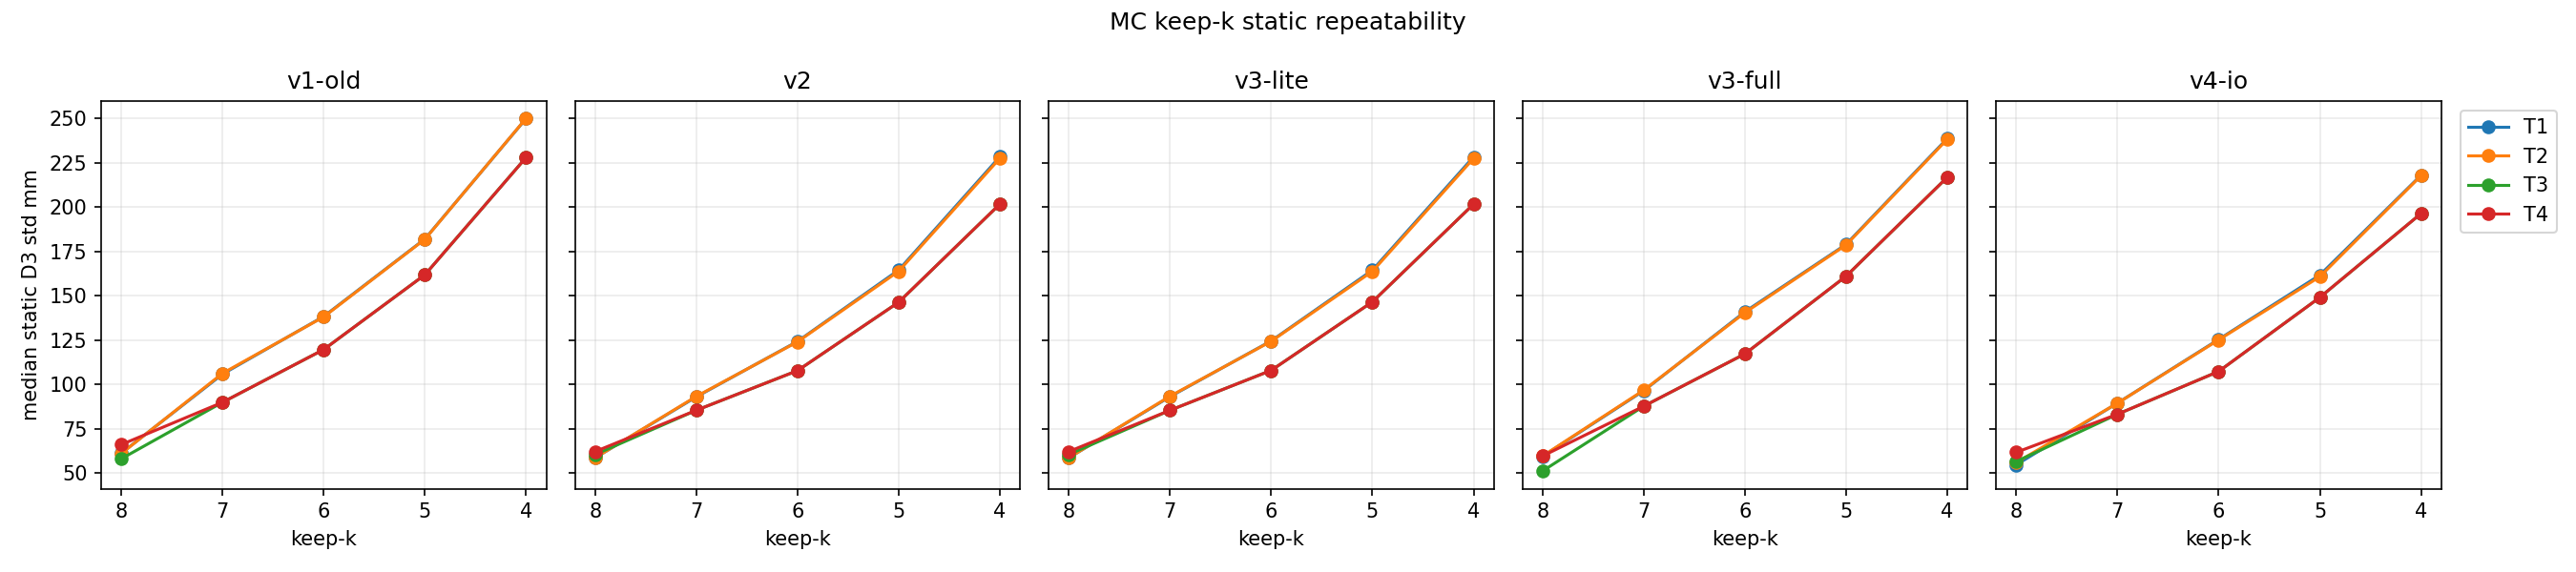
\includegraphics[width=\textwidth]{mc_keepk_static_curves.png}
\caption{Static keep-k}
\end{subfigure}
\begin{subfigure}{0.49\textwidth}
\centering
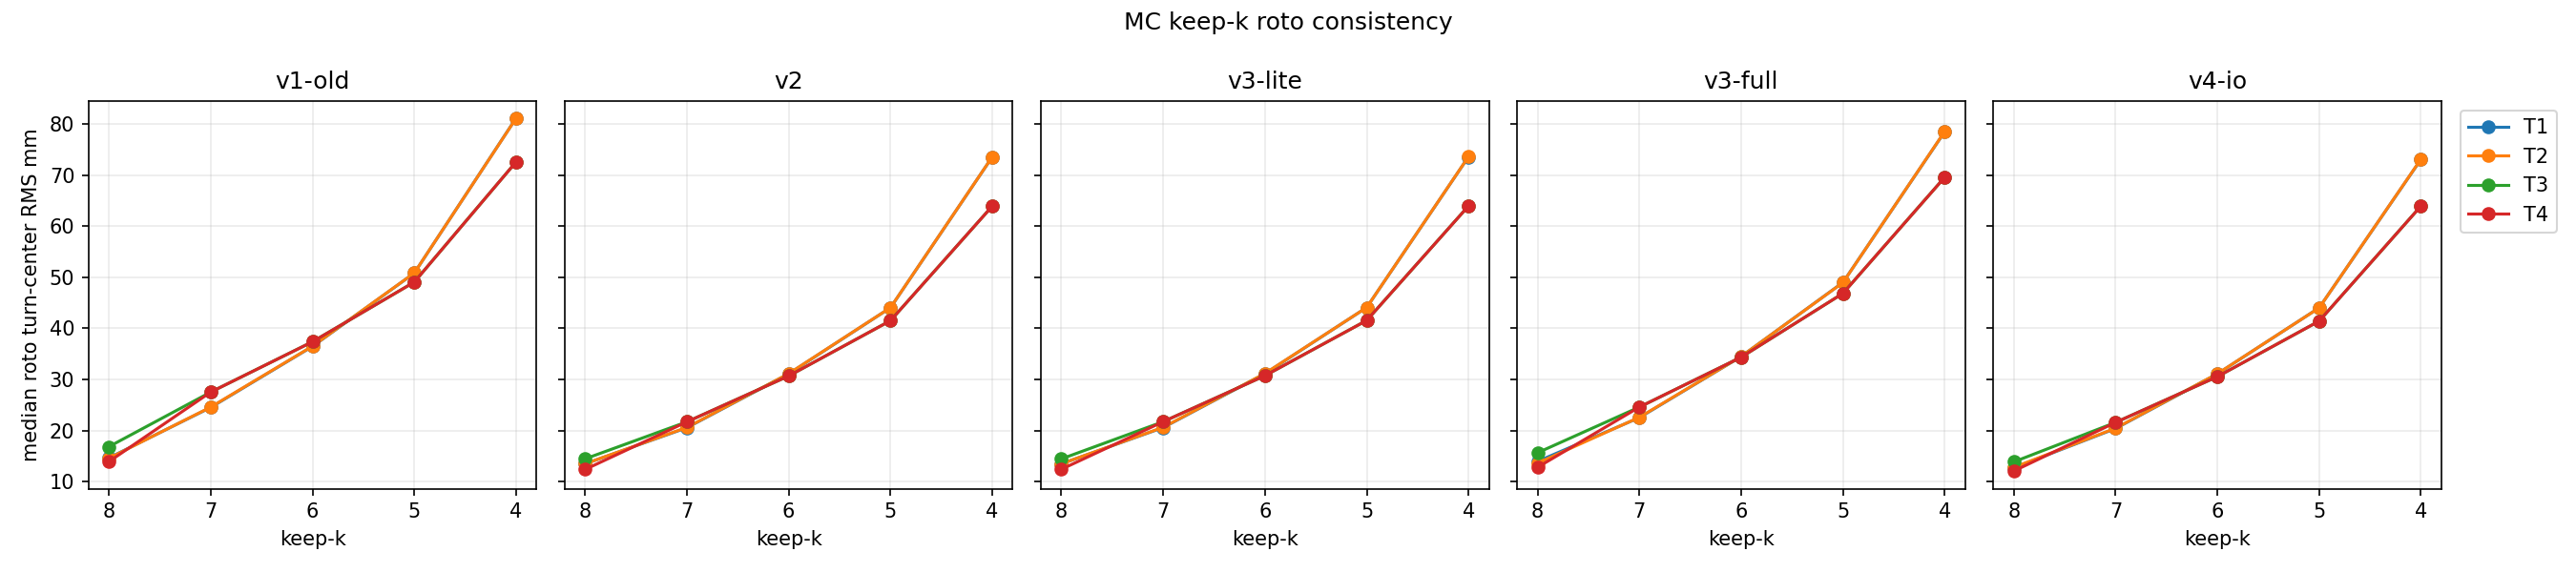
\includegraphics[width=\textwidth]{mc_keepk_roto_curves.png}
\caption{ROTO keep-k}
\end{subfigure}
\caption{Monte Carlo anchor-availability stress test. This belongs in a robustness section, not in the main accuracy headline.}
\end{figure}

\begin{figure}[H]
\centering
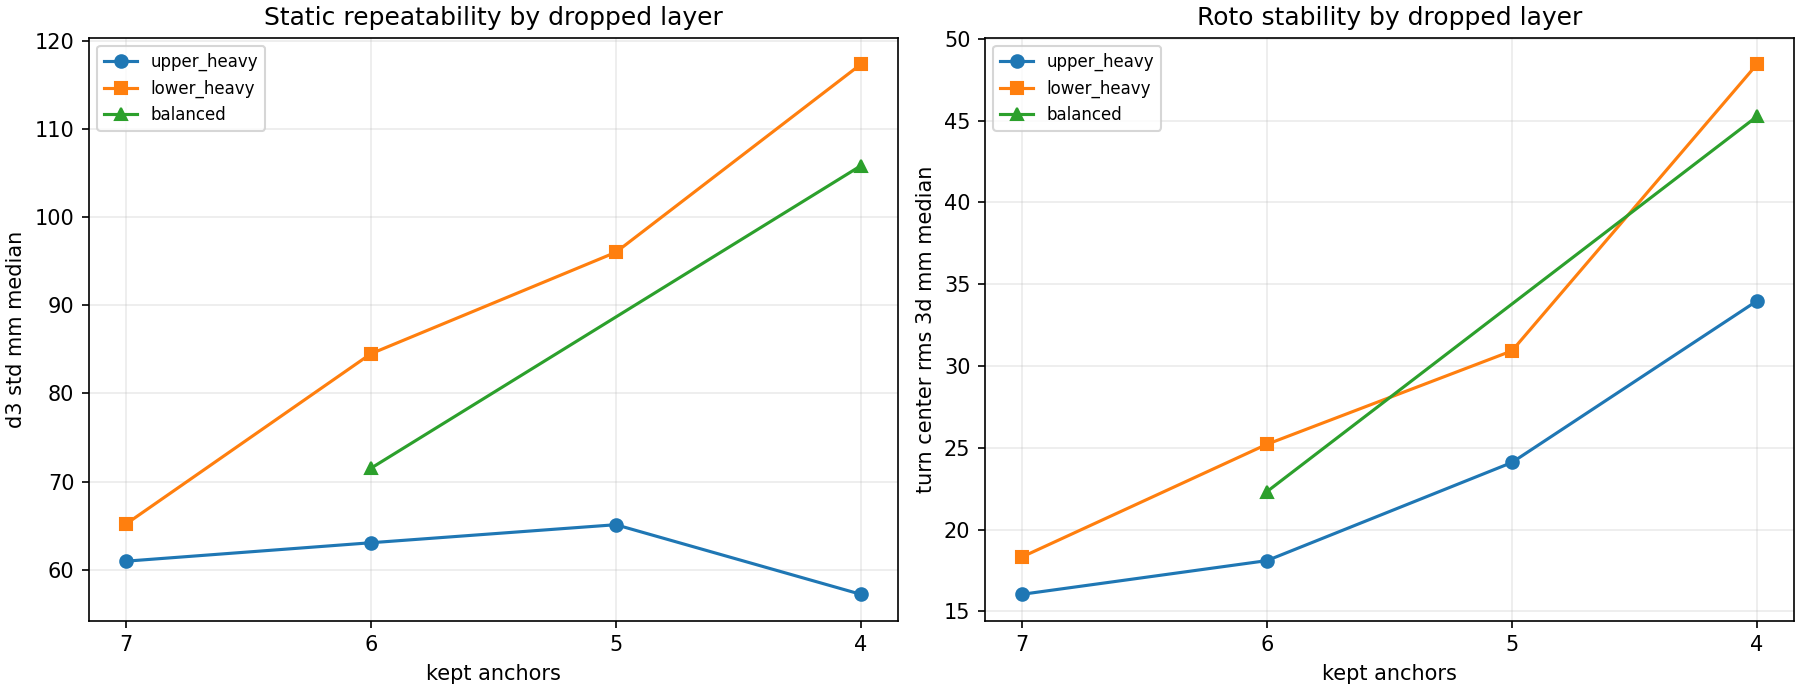
\includegraphics[width=0.72\textwidth]{stratified_keepk_upper_vs_lower.png}
\caption{Stratified upper/lower anchor removal. Removing lower-layer anchors is more damaging for the static metric.}
\end{figure}

For \case{v4-io/T4}, static repeatability $d_3$ standard-deviation median increases from $61.7\mm$ at keep8 to $83.2\mm$ at keep7, $107.3\mm$ at keep6, $149.1\mm$ at keep5, and $196.4\mm$ at keep4. ROTO turn-center RMS median increases from $12.1\mm$ at keep8 to $63.9\mm$ at keep4.

The stratified result is more informative than the aggregate curve alone. For static keep5, lower-heavy anchor drops reach $96.0\mm$ while upper-heavy drops reach $65.1\mm$; for keep4, lower-heavy drops reach $117.3\mm$ while upper-heavy drops are $57.2\mm$. The deployment lesson is that anchor count matters, but vertical and spatial coverage matter at least as much.

\section{Simulation and NLOS Discussion}

\begin{figure}[H]
\centering
\begin{subfigure}{0.49\textwidth}
\centering

\includegraphics[width=\textwidth]{wall_nlos_p95_comparison.png}
\caption{Wall distance versus P95 error}
\end{subfigure}
\begin{subfigure}{0.49\textwidth}
\centering

\includegraphics[width=\textwidth]{wall_nlos_convergence.png}
\caption{Convergence distance by material}
\end{subfigure}
\caption{Wall/NLOS simulation from \case{AutoPos_simulation}. It is useful for interpreting propagation risk, but it is not a substitute for the OptiTrack-referenced measurements.}
\end{figure}

\case{AutoPos_simulation} was produced after the measurement campaign and should be included as discussion or supplementary analysis. The wall/NLOS simulation shows a clear physical trend: clear LOS has about $0.062\m$ P95 error; the four-wall default case reaches about $0.764\m$, $0.287\m$, and $0.088\m$ at 0 cm, 40 cm, and 100 cm; the four-wall plus metal case reaches about $0.892\m$, $0.405\m$, and $0.123\m$ at the same distances. The extended convergence study suggests that the default wall needs about 115 cm to approach LOS+25\%, while wall plus metal needs about 145 cm.

This simulation supports the interpretation that wall proximity, metal, and obstruction can inflate the tail of the UWB localization error. It should be used to motivate CIR/NLOS detection and range weighting, not as a primary measured-performance result.

\section{Phase 4 UWB+IMU: L2/L16/L20 Sensor Comparison}

\begin{figure}[H]
\centering
\begin{subfigure}{0.49\textwidth}
\centering
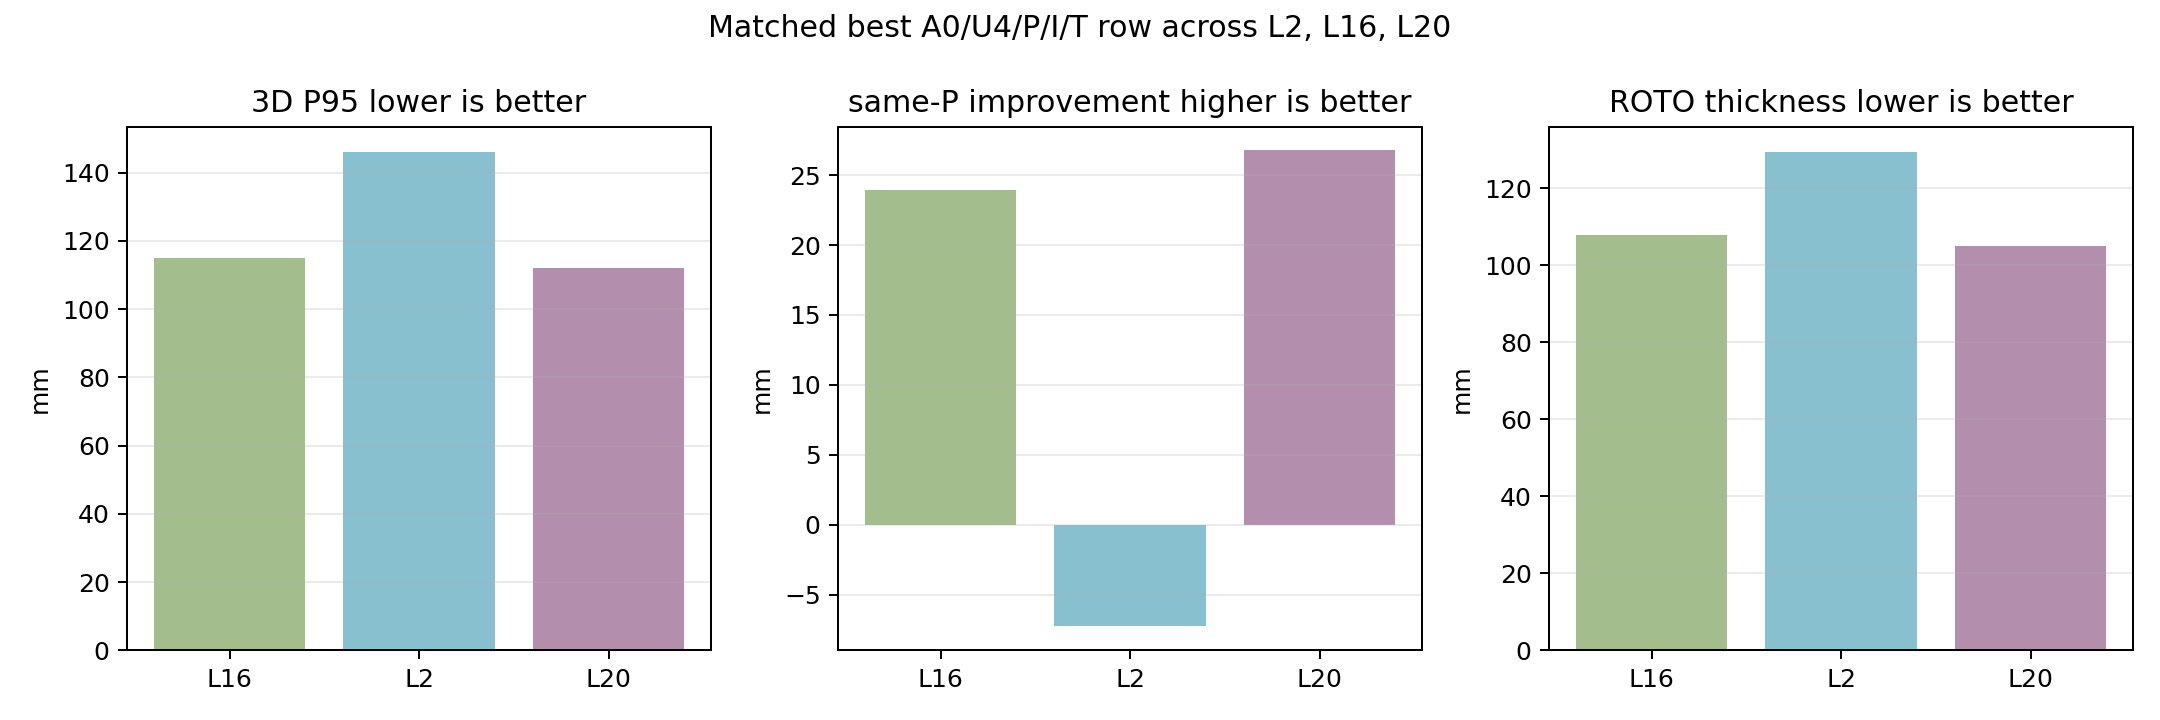
\includegraphics[width=\textwidth]{phase4_l2_l16_l20_sensor_comparison.png}
\caption{Matched best combo across sensors}
\end{subfigure}
\begin{subfigure}{0.49\textwidth}
\centering
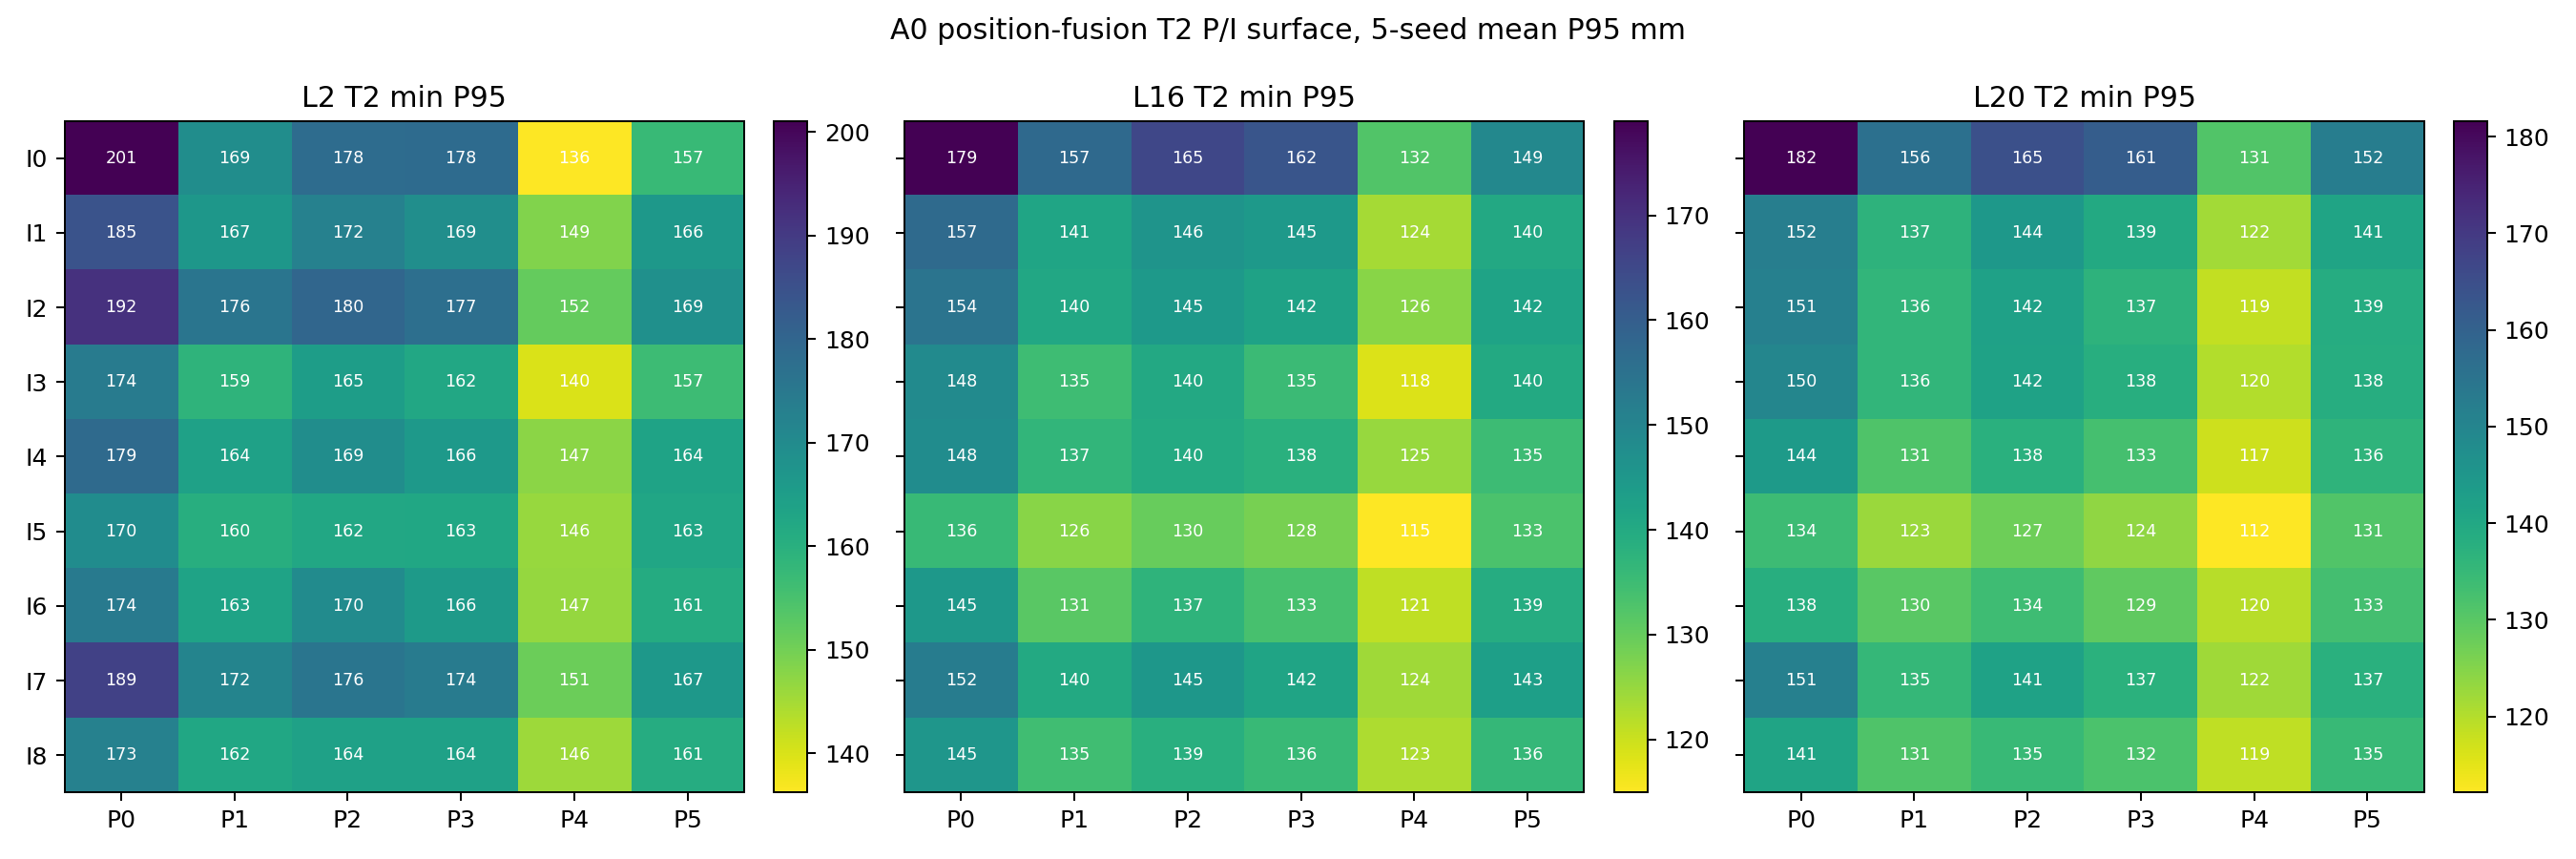
\includegraphics[width=\textwidth]{phase4_t2_pi_heatmap_by_sensor.png}
\caption{\case{T2} P/I heatmap by sensor}
\end{subfigure}
\caption{Phase 4 L2/L16/L20 TRUEFULL 5-seed Opti-truth analysis. Here L denotes the IMU sensor model, not the fusion algorithm.}
\end{figure}

This section should be based on the Phase 4 L2/L16/L20 TRUEFULL 5-seed Opti-truth analysis generated on 2026-06-05, not on the earlier real 6-axis vertical-slice smoke run. The Phase 4 run evaluates three IMU sensor models, L2, L16, and L20, with five seeds S00--S04 per sensor. Each seed contains 1377 runnable rows and is evaluated against the official ROTO Opti/Vicon trajectory tables. The production scope is A0; A1/A2/A3 are control or oracle layouts and should not be used for production recommendations.

The three sensor models are:
\begin{itemize}
\item \case{L2}: MPU6050/JY61P-like 6-axis IMU, representing a low-cost 6-axis baseline.
\item \case{L16}: InvenSense ICM-45686 premium 6-axis IMU, representing a high-performance consumer/robotics-grade 6-axis candidate.
\item \case{L20}: Xsens/Movella MTi-3-5A-T industrial AHRS module, simulated here as accel+gyro, representing an industrial-quality IMU candidate.
\end{itemize}

The Phase 4 headline row is \case{X_A0_U4_P4_L20_I5_T2}. Its 5-seed mean track-median 3D P50/P95/RMSE is $68.4/112.1/75.7\mm$. The same-P UWB P95 is $138.9\mm$, so the same-P P95 improvement is $26.8\mm$; the improvement over B0 P0 is $119.7\mm$; and the ROTO radius abs / band P95 is $16.6/105.1\mm$. This means the IMU is not only rescuing a failed system. On top of a strong P4 UWB branch, it still reduces the dynamic tail and improves ROTO shape metrics.

\begin{table}[H]
\centering
\caption{Phase 4 matched best combo across sensors. All errors are in mm and are 5-seed means.}
\begin{tabular}{@{}l l r r r r r r@{}}
\toprule
Sensor & Best matched row & P50 & P95 & RMSE & same-P $\Delta$P95 & Radius abs & Band P95 \\
\midrule
L20 & \case{X_A0_U4_P4_L20_I5_T2} & 68.4 & 112.1 & 75.7 & 26.8 & 16.6 & 105.1 \\
L16 & \case{X_A0_U4_P4_L16_I5_T2} & 69.0 & 114.9 & 76.1 & 23.9 & 16.9 & 107.8 \\
L2 & \case{X_A0_U4_P4_L2_I5_T2} & 83.9 & 146.2 & 94.2 & -7.3 & 20.1 & 129.6 \\
\bottomrule
\end{tabular}
\end{table}

The ranking is clear: L20 is best, L16 is very close, and L2 is weaker in aggregate precision. The L2 matched row even has a negative same-P P95 delta of $-7.3\mm$. This should not be interpreted as ``L2 is useless.'' It means that the matched-best L2 row is not a good incremental improvement over the strong P4 baseline. Other L2 rows and the spiky-track rescue still show that a low-cost IMU can remove large dynamic jumps.

\subsection{Production A0 Baseline and IMU Improvement Modes}

The Phase 4 report also gives production A0/U4 UWB baselines by P. The P4 baseline is already strong, with P50/P95/RMSE of $78.2/138.9/86.2\mm$. The P0 raw UWB branch is much worse at $105.8/231.8/132.8\mm$. Therefore, UWB+IMU has two distinct improvement modes:
\begin{enumerate}
\item \textbf{Incremental improvement over a strong UWB baseline:} the best L20 row reduces P4 P95 from $138.9\mm$ to $112.1\mm$, an improvement of $26.8\mm$.
\item \textbf{Rescue from raw or weak UWB:} \case{X_A0_U4_P0_L20_I5_T2} reaches $133.9\mm$ P95, improving over same-P P0 UWB by $97.9\mm$.
\end{enumerate}

These two claims should remain separate. The first is about raising the ceiling of the best UWB pipeline; the second is about suppressing large dynamic failures in weaker UWB branches.

\subsection{Same Spiky Track Comparison}

\begin{figure}[H]
\centering

\includegraphics[width=0.82\textwidth]{phase4_spiky_track_xz_l2_l16_l20.png}
\caption{Professor-view spiky track comparison on \case{R01/BS2DCE}. This track was selected because B0 pure UWB has the most X-Z jump spikes in the ROTO set.}
\end{figure}

\begin{figure}[H]
\centering
\begin{subfigure}{0.49\textwidth}
\centering

\includegraphics[width=\textwidth]{phase4_spiky_track_err3d_l2_l16_l20.png}
\caption{3D error over time}
\end{subfigure}
\begin{subfigure}{0.49\textwidth}
\centering
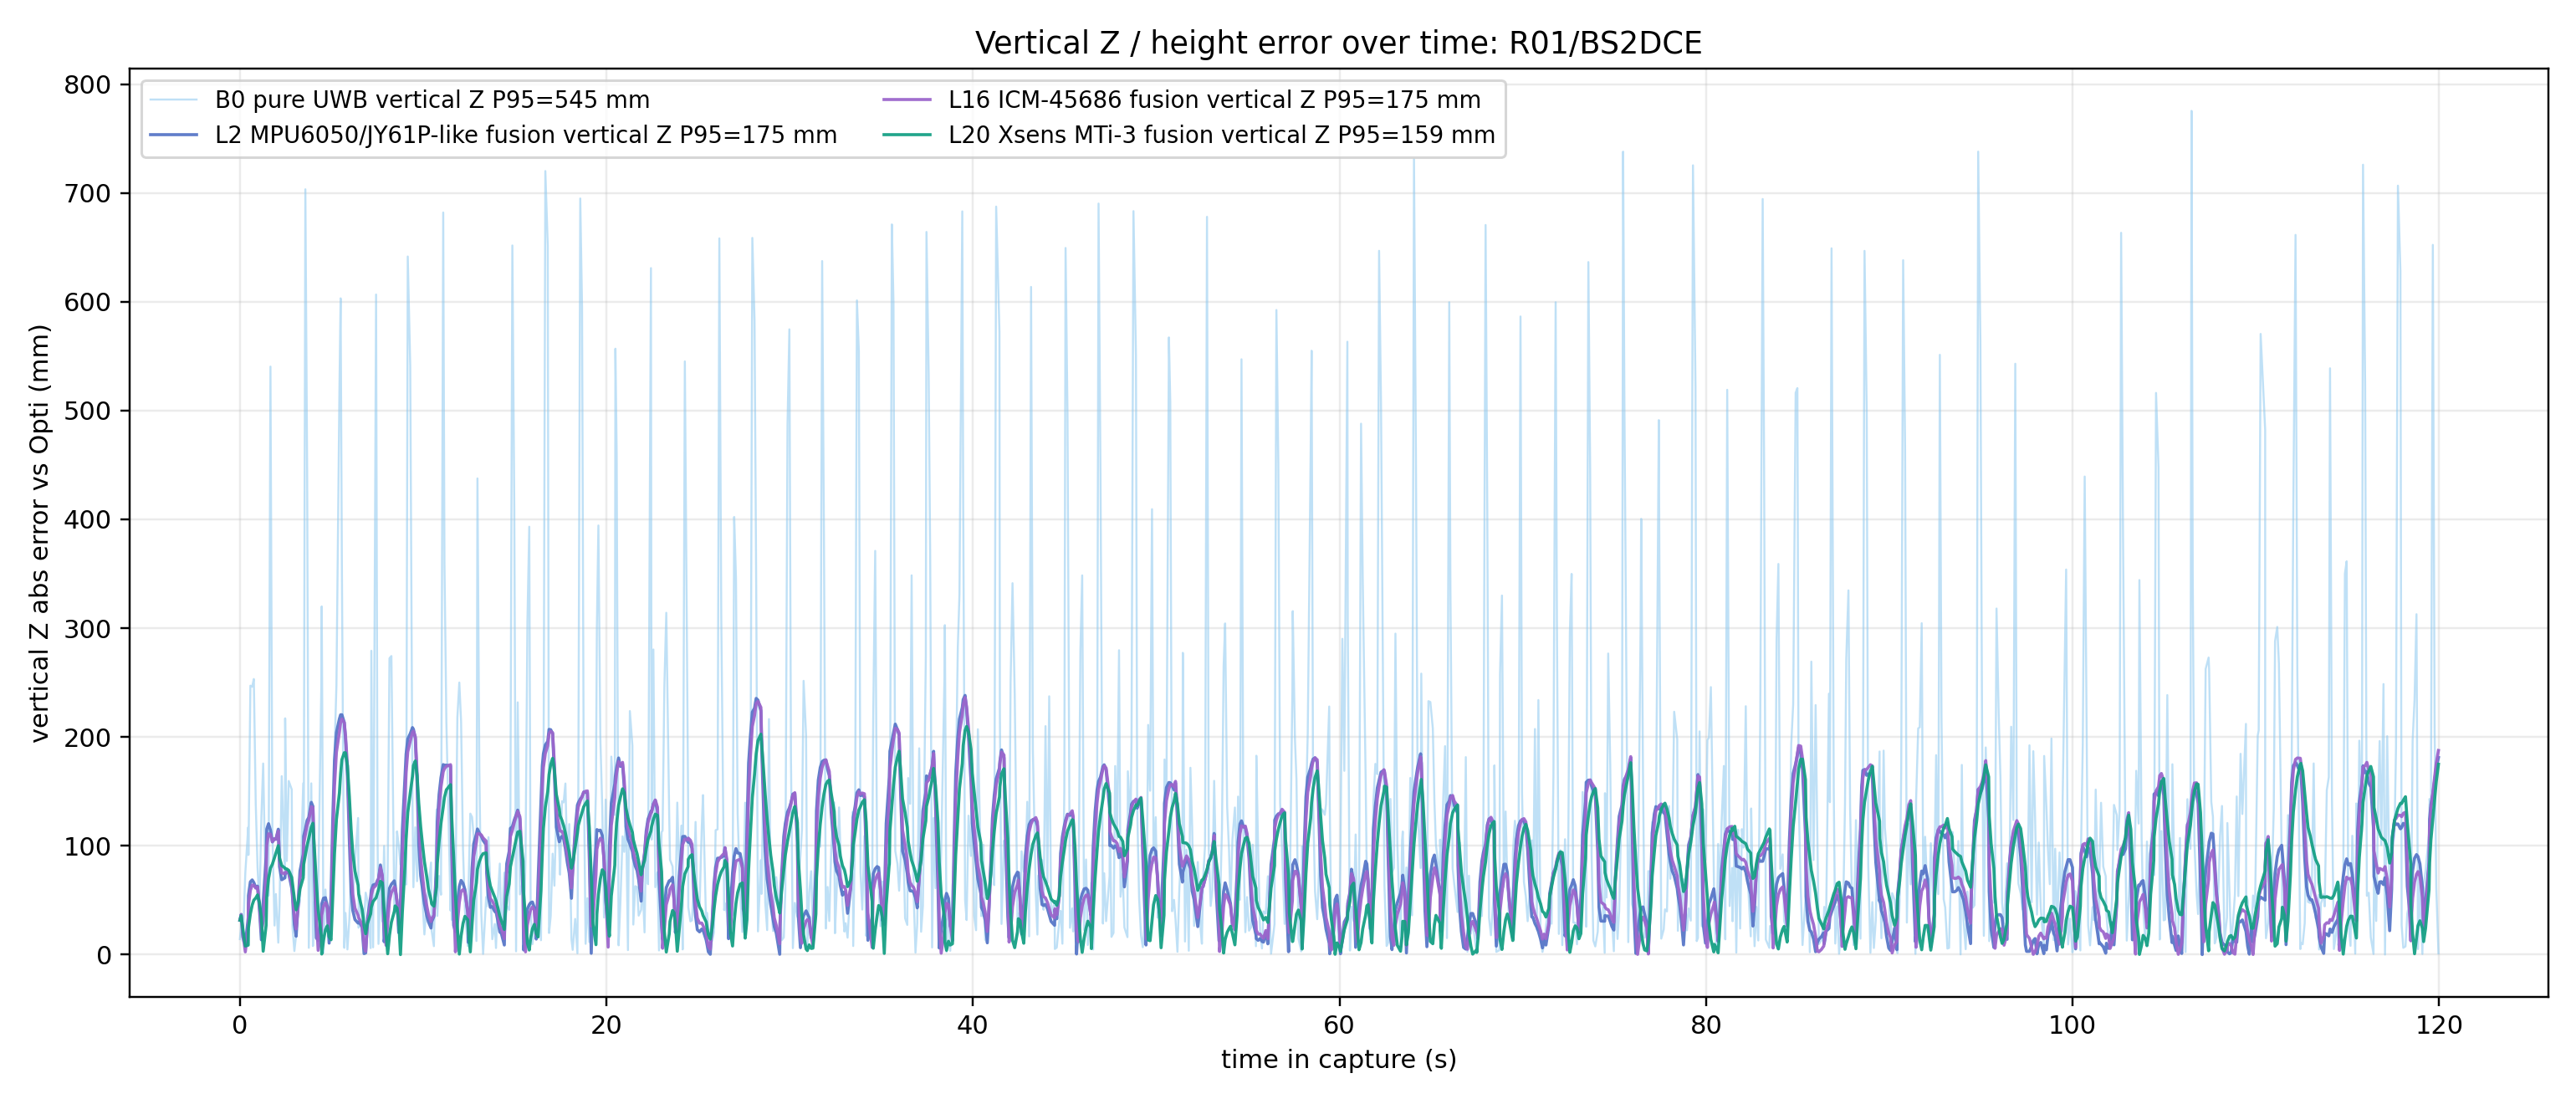
\includegraphics[width=\textwidth]{phase4_spiky_track_vertical_l2_l16_l20.png}
\caption{Vertical Z error over time}
\end{subfigure}
\caption{Error time series on the same spiky track. The presentation labels the height axis as Vertical Z; internally this uses the official aligned table's \case{y_vertical} height column.}
\end{figure}

The spiky-track comparison is especially useful for the report because it shows what IMU fusion fixes visually and temporally. On \case{R01/BS2DCE}, B0 pure UWB has 178 samples with X-Z jumps greater than $200\mm$, a jump p99 of $425.8\mm$, a maximum jump of $506.5\mm$, a 3D P95 of $595.5\mm$, and a vertical Z P95 of $545.1\mm$. After fusion, all three IMU cases reduce the X-Z jump $>200\mm$ count to zero:
\begin{itemize}
\item \case{L2}: \case{X_A0_U4_P4_L2_I5_T3}, fusion 3D P95 $188.4\mm$, improvement over B0 $407.0\mm$, vertical Z P95 $175.4\mm$.
\item \case{L16}: \case{X_A0_U4_P4_L16_I6_T4}, fusion 3D P95 $185.1\mm$, improvement over B0 $410.4\mm$, vertical Z P95 $175.1\mm$.
\item \case{L20}: \case{X_A0_U4_P4_L20_I3_T2}, fusion 3D P95 $169.4\mm$, improvement over B0 $426.0\mm$, vertical Z P95 $159.3\mm$.
\end{itemize}

This should be written as a strong dynamic-result claim: the primary value of IMU fusion is not only improving static point accuracy; it suppresses discrete UWB-only jumps and vertical spikes in dynamic ROTO. Even L2, although weaker in the aggregate matched-best table, removes all large X-Z jumps on the selected spiky track.

\subsection{Stress Test Robustness}

\begin{figure}[H]
\centering
\begin{subfigure}{0.49\textwidth}
\centering
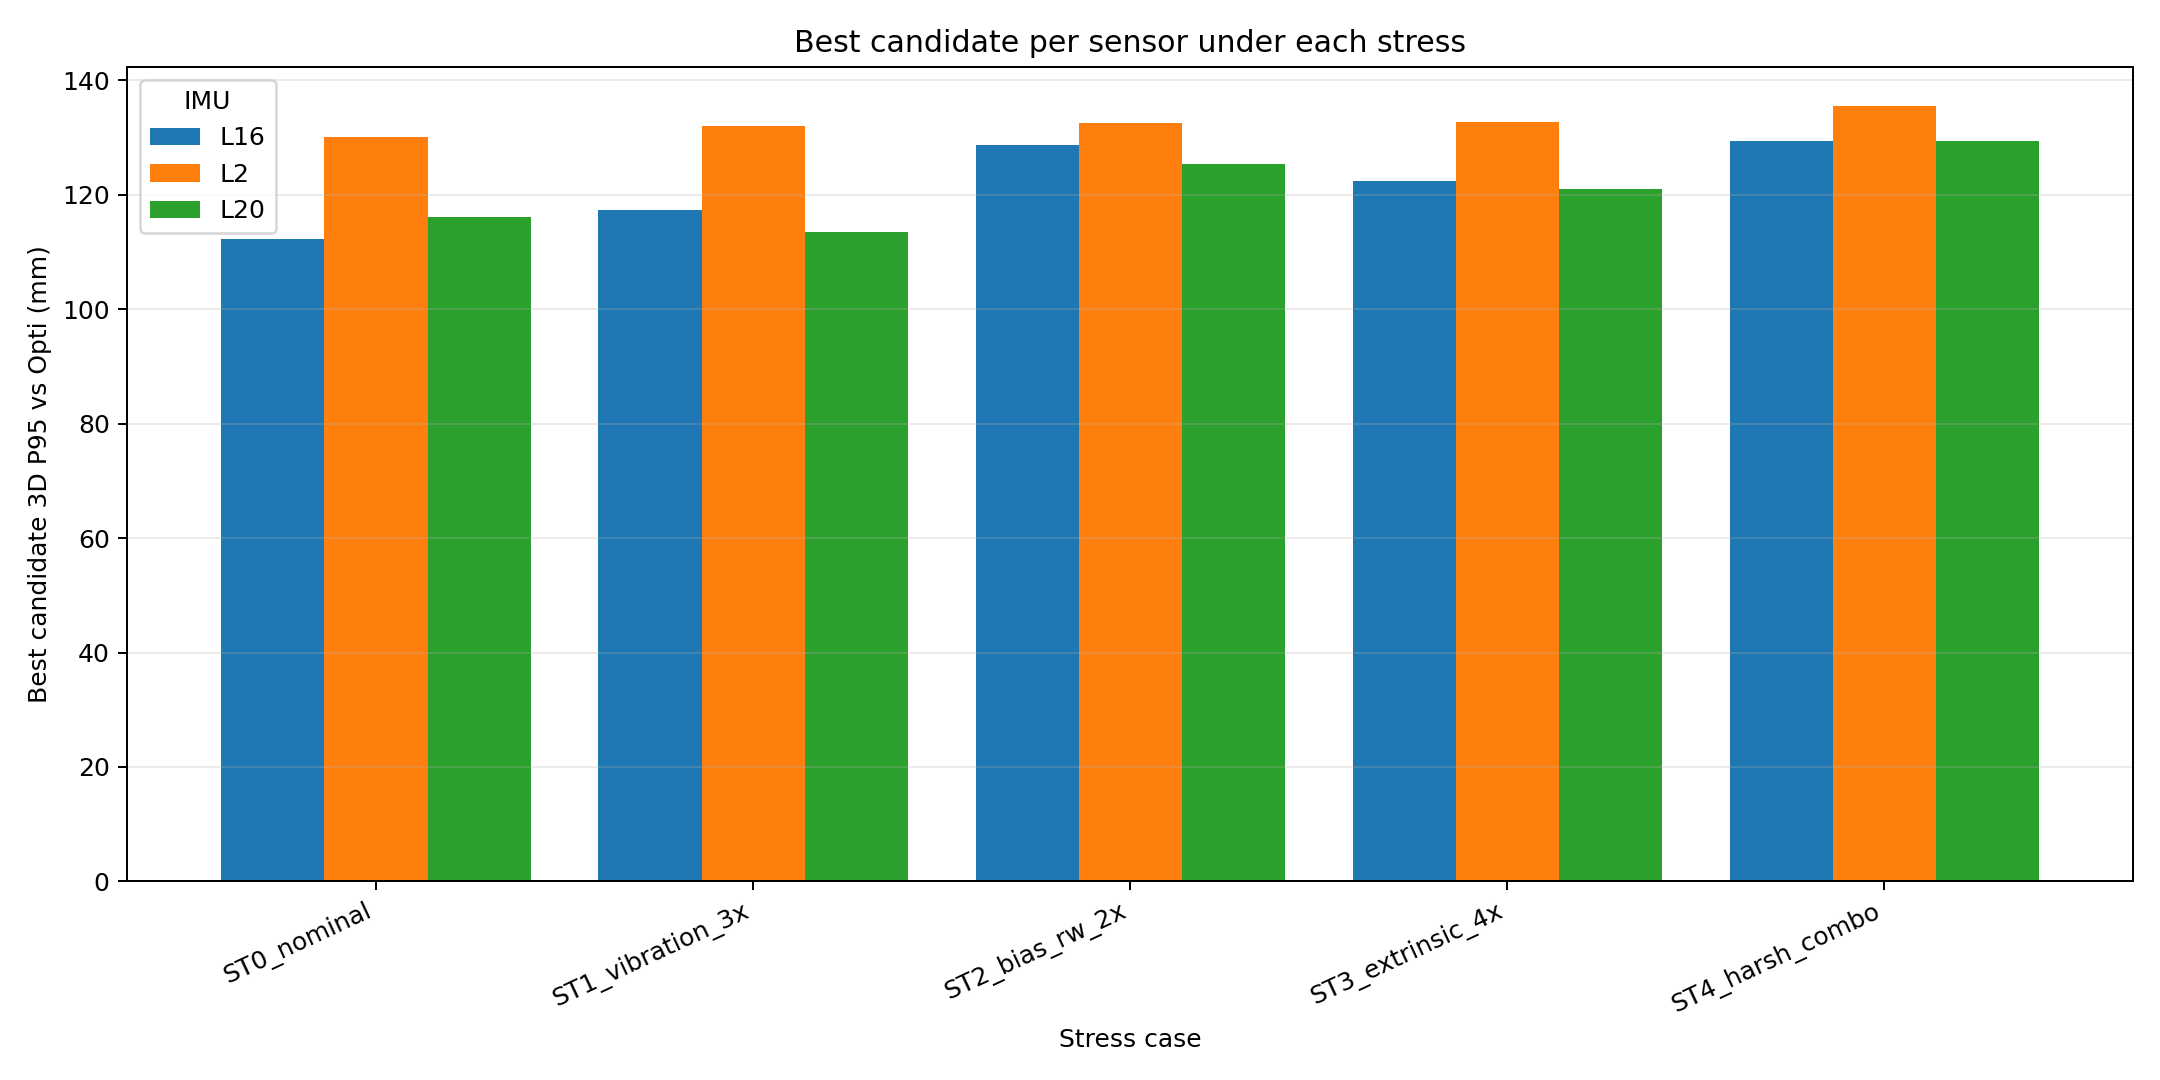
\includegraphics[width=\textwidth]{imu_stress_best_per_sensor_p95.png}
\caption{Best row per sensor and stress}
\end{subfigure}
\begin{subfigure}{0.49\textwidth}
\centering
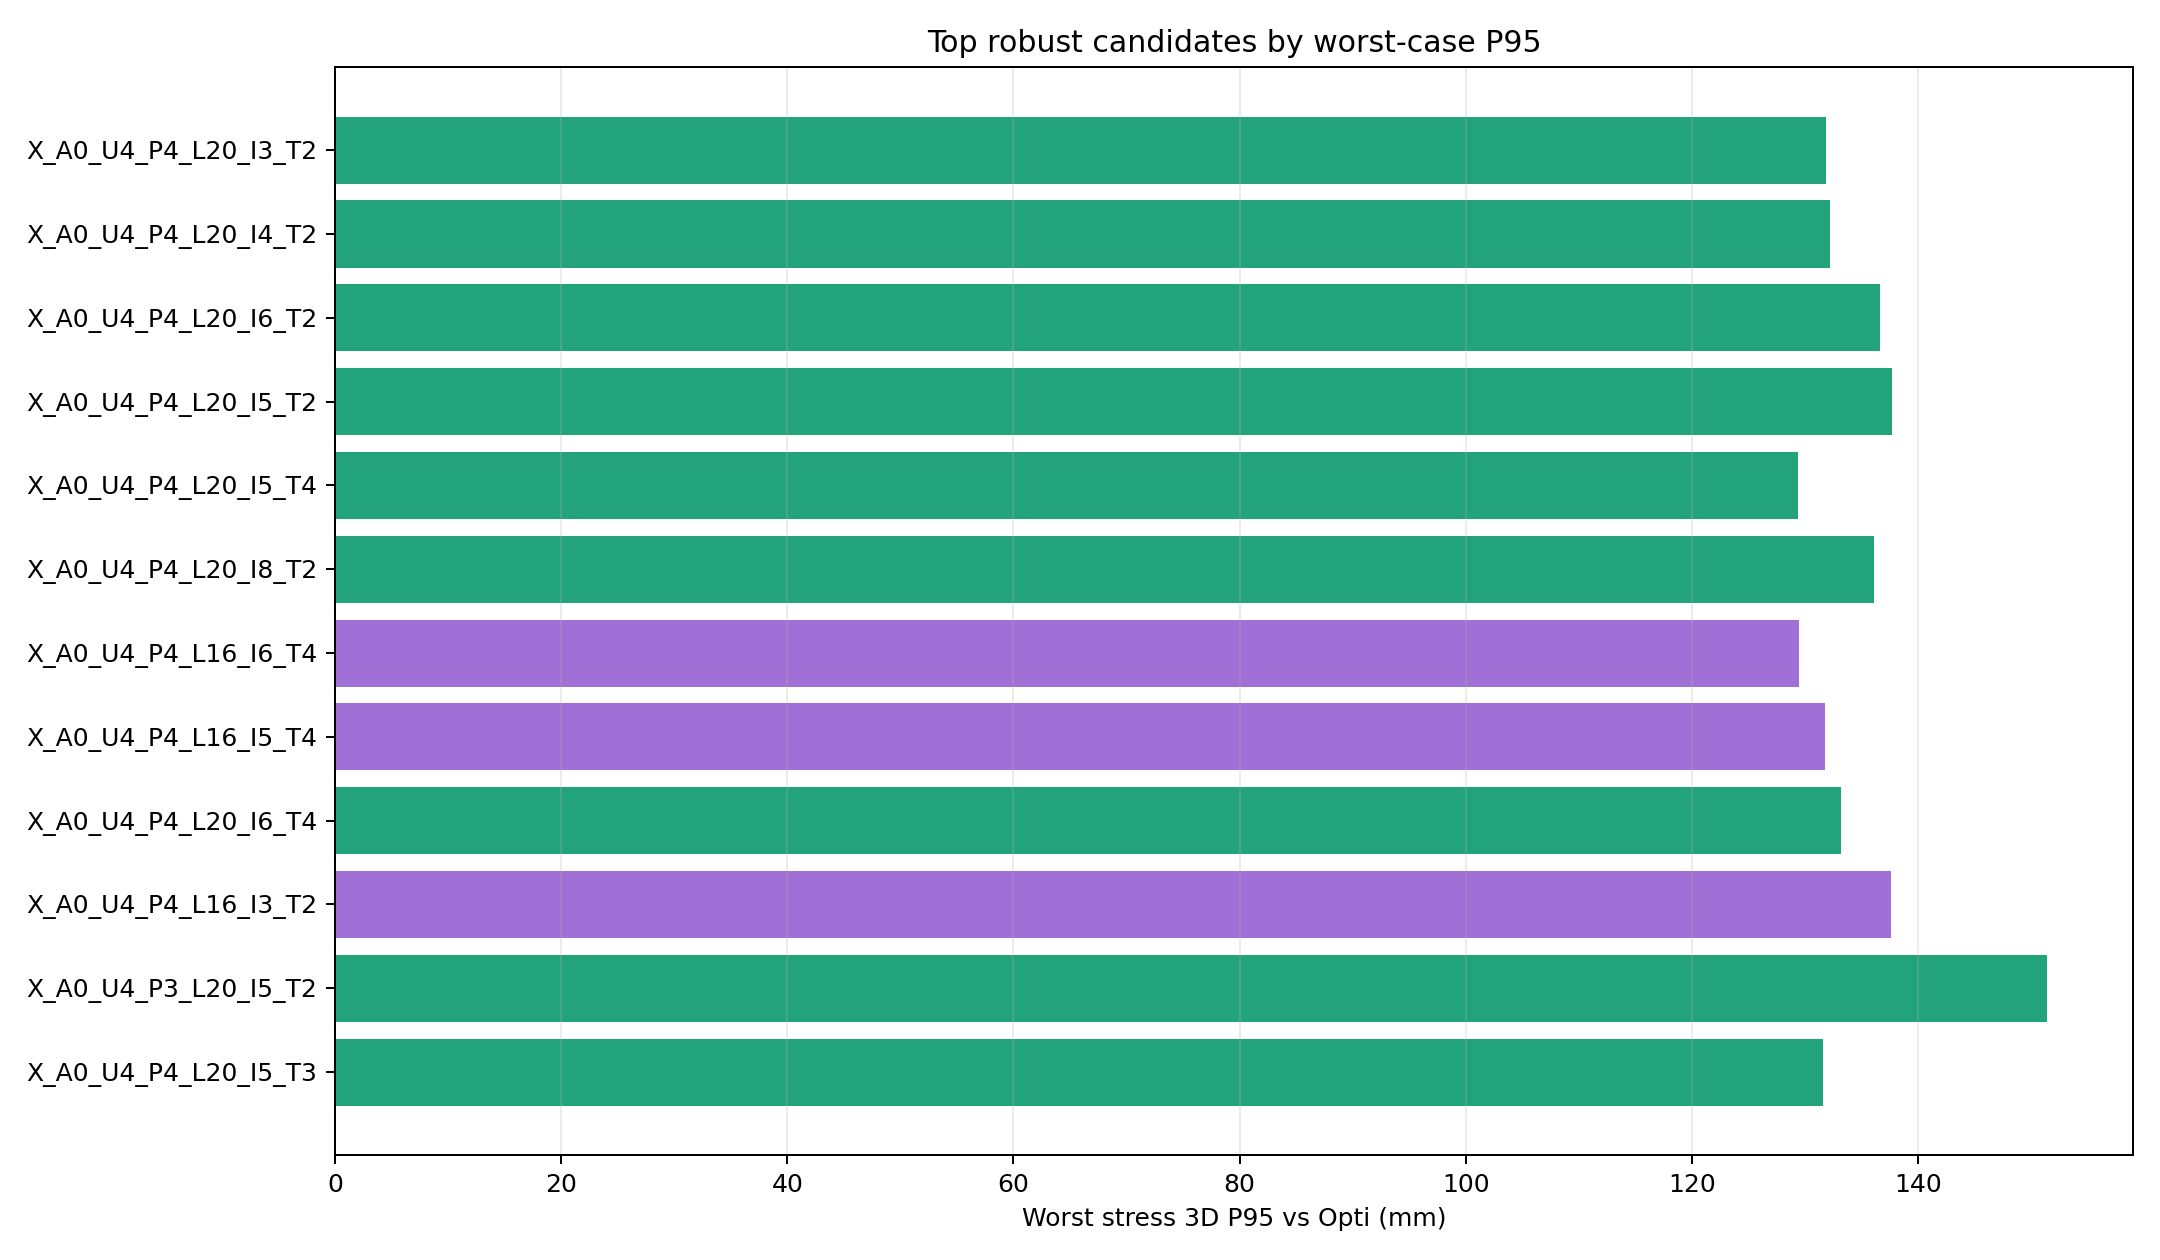
\includegraphics[width=\textwidth]{phase4_stress_top12_worstcase_p95.png}
\caption{Top12 worst-case P95 ranking}
\end{subfigure}
\caption{Phase 4 L2/L16/L20 stress candidate test. Stress cases include vibration, bias random walk, extrinsic residual, and a harsh combined case.}
\end{figure}

The stress candidate test covers five cases: \case{ST0_nominal}, \case{ST1_vibration_3x}, \case{ST2_bias_rw_2x}, \case{ST3_extrinsic_4x}, and \case{ST4_harsh_combo}. The robust top ranks are dominated by L20. Robust rank 1 is \case{X_A0_U4_P4_L20_I3_T2}, with mean P95 $124.1\mm$, worst P95 $131.9\mm$, and mean same-P improvement $14.8\mm$. The best L16 robust row appears at rank 7, \case{X_A0_U4_P4_L16_I6_T4}, with mean/worst P95 of $129.1/129.5\mm$. L2 is generally behind L16/L20, but its best rows under stress remain around $130$--$136\mm$ P95, which means the low-cost sensor is weaker in ceiling performance rather than completely unusable.

The engineering conclusion is direct: if the goal is best dynamic performance and robustness, the L20/Xsens-like industrial IMU is the current Phase 4 winner. If cost, size, and procurement matter, L16/ICM-45686 is very close and may be the more realistic high-performance 6-axis candidate. L2/MPU6050-like is a useful low-cost baseline; it is weaker in aggregate precision, but it still has clear rescue value against extreme UWB spikes.

\subsection{Raw-range Branch Is Not Recommended Yet}

The Phase 4 raw-range branch should be reported as a negative control. The best raw row, \case{X_A0_R4_L20_I5_T10}, has P95 $465.4\mm$ and B0 delta $-233.6\mm$, so it is substantially worse than B0 in the current proxy implementation. The practical path is therefore position-branch fusion on \case{A0/U4/Px}, not the current raw-range branch.

\subsection{IMU Claim and Boundary}

IMU should no longer be described only as future work. A better statement is: \textbf{Phase 4 replay/simulation evidence shows that UWB+IMU can reduce ROTO P95, suppress spiky jumps, and distinguish sensor-model value across L2/L16/L20.} At the same time, this is still an Opti-truth evaluated simulation/replay sweep, not a fully embedded real-time Ghost IMU deployment. The main report should keep UWB-only OptiTrack validation as the primary result, then present IMU as the strongest next dynamic-extension result.

\section{CIR: Future Work Only For Now}

CIR should not be presented as a result section yet. At the moment, there is no complete aligned CIR/NLOS label table or reproducible CIR metric in the main analysis chain. CIR is best framed as future work: LOS/NLOS classification, dynamic range weighting, multipath rejection near walls and metal, and fusion with an IMU motion prior.

\section{Recommended Report Structure}

A final written report can follow this structure:
\begin{enumerate}
\item Introduction: validate AutoPos UWB self-deployment and tag localization, not just one solver number.
\item Dataset and Coordinate Systems: OptiTrack, AutoPos layout, static replay, and ROTO.
\item AutoPos Anchor Layout: SE(3) and Sim(3) layout error.
\item Delay-layout Coupling: the four control cases showing why delay must match layout.
\item Static Tag Localization: production \case{v4-io/T4} at $72.7/171.5/109.8\mm$.
\item Dynamic ROTO Evaluation: \case{v4-io/T4} at $105.8/231.8/141.3\mm$ and why timing alone cannot explain the error.
\item Robustness and Simulation: Monte Carlo keep-k and wall/NLOS simulation.
\item Phase 4 UWB+IMU and Future CIR: detailed L2/L16/L20 dynamic-fusion evidence, with CIR kept as future work.
\item Limitations: single site, OptiTrack dependence, missing CIR/NLOS labels, and IMU not yet fully closed-loop.
\item Conclusion: usable self-localization, delay-layout coupling, dynamic propagation challenges, and next-step roadmap.
\end{enumerate}

\section{Conclusion}

The strongest conclusion from the Erlangen official dataset is that AutoPos UWB self-localization provides a usable anchor geometry and enables approximately 7--11 cm-level static tag localization in a real measured field setup. However, deployed UWB accuracy is not determined by geometry alone. Layout, delay calibration, solver choice, motion state, and propagation environment must be treated together. The production \case{v4-io/T4} static result should be the headline; ROTO should be presented as the dynamic challenge; Monte Carlo and wall/NLOS simulation should support robustness and error-source discussion; IMU and CIR should be framed as the next engineering path, with IMU already showing preliminary promise and CIR still requiring aligned labels and metrics.

\end{document}
